% JKAIA 2026 (2026 한국인공지능학회 추계학술대회) -- General (Poster) 트랙, 한국어 작업본
% ※ 제출본은 영문 main.tex다. 이 파일은 저자가 내용을 검토·수정하기 위한 한국어 대조본이며, 문단 구조가 main.tex와 1:1로 같다.
%    이 파일을 고치면 같은 자리의 영문을 main.tex에 반영한다.
% 템플릿: kaia.cls (2026-10 배포본, 10pt, A4). 포스터 트랙은 이 템플릿으로 1~2쪽 요약본을 낸다.
% 심사는 single-blind이므로 저자를 명기한다.
%
% 학회 논문제출 안내: "제출 논문은 영문으로 작성" (2026-10-15 확인) → 영문 main.tex를 제출한다.
%
% 빌드: tectonic -X compile main.tex  (XeTeX: 한글은 kotex/xetexko + Apple SD Gothic Neo)
%      pdflatex 사용 시에는 kotex(kotex-utf)와 나눔 Type1 폰트가 필요하다.
%
% 템플릿 대비 변경점:
%  * 템플릿의 \fbox{\parbox}는 쪽을 넘기지 못하므로 두 쪽 요약을 위해 mdframed로 같은 테두리를 그린다.
%  * kaia.cls의 \maketitle이 \twocolumn[...]을 호출하므로 \twocolumn을 1단으로 재정의해 템플릿 PDF와 같은 1단을 유지한다.
%  * XeTeX에서는 Times(mathptmx)가 매핑되지 않아 시스템 Times New Roman을 쓴다.

\documentclass[nouppercase]{kaia}
\usepackage{amsmath}
\usepackage{booktabs}
\usepackage{graphicx}
\usepackage[framemethod=TikZ]{mdframed}
\usepackage{iftex}
\ifXeTeX
  \usepackage{fontspec}
  \setmainfont{Times New Roman}
  \usepackage{kotex}
  \setmainhangulfont{Apple SD Gothic Neo}[BoldFont={* Bold}, ItalicFont={* Light}]
\else
  \usepackage{kotex}
\fi
\usepackage{multicol}
\makeatletter
\newenvironment{posterrefs}{\par\vspace{2pt}\noindent{\small\textbf{References}}\par
  \def\@openbib@code{\scriptsize\setlength{\itemsep}{0pt}\setlength{\parsep}{0pt}\setlength{\topsep}{0pt}}%
  \let\section\@gobbletwo
  \setlength{\multicolsep}{0pt}\vspace{-0.8\baselineskip}%
  \begin{multicols}{2}\begin{thebibliography}{7}}{\end{thebibliography}\end{multicols}}
\makeatother
\graphicspath{{../figures/}{../../report/figures/}}

\makeatletter
\renewcommand{\twocolumn}[1][]{#1}   % 1단 유지; \maketitle의 선택 인자는 그대로 조판된다
\makeatother
\mdfsetup{linewidth=0.4pt, linecolor=black, innerleftmargin=7pt, innerrightmargin=7pt,
          innertopmargin=4pt, innerbottommargin=4pt, skipabove=4pt, skipbelow=4pt}

\title{고정된 주행 World-Action Model의 첫 상상 패스에서 읽어내는 경량 행동 예측\\[2pt]
{\normalsize\normalfont Imagine Once, Act Fast: Lightweight Action Readout from a Frozen Driving World-Action Model}}

\author{송용휘}{a}
\author{강현수}{a}
\affiliation{충북대학교 정보통신공학부, 청주, 대한민국, \{thddydgnl1937@gmail.com, hskang@chungbuk.ac.kr\}}{a}

\begin{document}

\maketitle
\vspace{-28pt}

\begin{mdframed}

\begin{abstract}
DriveWAM과 같은 주행 World-Action Model(WAM)은 5B 비디오 확산 트랜스포머로 미래 영상 잠재(latent)를 상상한 뒤, 같은 백본을 10회 더 실행해 4초 행동 chunk를 denoising하며, 이것이 추론 지연의 가장 큰 항이다. 본 연구는 고정된 백본의 첫 미래 denoising 패스(미래 패스 1) 직후 표현에서 작은 head가 궤적을 읽어낼 수 있는지 묻는다. 이 패스에서 세 트랜스포머 블록을 hook으로 읽고, 1천만 파라미터의 state-fusion head(SF3)로 궤적을 회귀한 뒤 추론을 종료한다. 공개 checkpoint는 갱신하지 않는다. NAVSIM에서는 공식 DriveWAM보다 4.2배, 품질을 유지하는 가장 빠른 저단계 기준보다 2.2배 빠르면서 PDMS 손실은 0.2--0.4점이다. NVIDIA PhysicalAI-AV 공식 test에서는 11.8배 빠르면서 궤적 오차가 DriveWAM과 비슷하다. 공식 단일 표본보다는 낮고, dev 세트에서 표본 4개 평균과 비교하면 ADE는 대등, FDE는 약 0.1 m 높다. 진단 결과 미래 패스 1에 행동 정보 대부분이 이미 들어 있고, 미래 denoising을 더 해도 유의한 이득이 없으며, head 학습 데이터가 늘수록 격차가 꾸준히 줄었다.
\end{abstract}
\begin{keywords}
World-action model, 자율주행, 효율적 추론, 비디오 확산 모델, 궤적 계획
\end{keywords}

\subsection{문제 정의}
DriveWAM~\cite{shi2026drivewam}(6.24B 파라미터, Wan2.2-TI2V-5B~\cite{wan2025wan} 기반)은 자기회귀 video-action 정책이다. 과거 프레임, ego 상태, 안내 문장을 조건으로 미래 영상 잠재를 확산 트랜스포머 3패스로 denoising한 뒤, 4초 행동 chunk를 같은 트랜스포머 10패스로 denoising한다(B10). 본 연구는 백본을 재학습하지 않고, 미래 생성의 어느 시점, 어느 깊이에서 행동을 한 번에 읽어낼 수 있는지 묻는다. 품질은 B10, 그리고 개발(dev) 세트에서 B10 품질을 유지하는 가장 빠른 저단계 변형 $B^{*}$와 비교한다. 단계를 줄이는 데는 학습이 필요 없기 때문이다.

\subsection{독창성}
(1) \textit{고정된 WAM 자신의 상상에서 읽기.} Light-WAM~\cite{li2026lightwam}과 두 Faster-WAM 연구~\cite{ma2026fasterwam,zhao2026fasterwam}는 가벼운 action expert와 함께 백본을 학습하거나 적응시킨다. 본 연구는 공개 DriveWAM checkpoint를 고정한 채 행동 생성기만 교체하고 미래 패스 1에서 백본을 읽는다. 기여는 head 구조가 아니라 언제, 어디서 읽느냐에 있다. (2) \textit{세 가지 읽기 시점}: \texttt{current}, \texttt{first}, \texttt{terminal}(표~\ref{tab:diag}). (3) \textit{사전등록 평가}: 분할, $B^{*}$ 선정, 품질 임계값, head 사양을 결과를 보기 전에 고정했고 잠금 final 세트는 1회만 평가했다. (4) \textit{평가 함정 두 가지}: 공개 NAVSIM 백본은 학습 장면을 기억하고 있고(B10 ADE navtrain 0.076 m 대 navtest 0.598 m), PhysicalAI single-seed protocol은 seed에 민감하다(B10 dev ADE 0.82--0.93 m).

\subsection{알고리즘}
\textbf{고정 백본과 표현 추출.} 공식 추론 루프를 재구현해 원본과 비트 단위로 같음을 확인했고, forward hook으로 블록 10, 20, 30을 읽는다. \texttt{first} 표현을 쓰면 미래 패스 1 직후 추론을 끝낸다(그림~\ref{fig:overview}).
\textbf{SF3 head}(998만 파라미터, 백본의 0.16\%). head는 Light-WAM action expert의 다층 state-fusion 설계(블록당 학습 query 16개, 융합 MLP, step별 디코딩)를 따른다~\cite{li2026lightwam}. 다른 점은 붙는 대상과 예측하는 것이다. 고정된 DriveWAM 백본에 head만 따로 학습하고, 관측이 아니라 미래 패스 1을 읽으며, ego 상태를 입력으로 받아 step별 정규화 변위와 heading을 낸다(NAVSIM 2 Hz 8 pose, PhysicalAI 10 Hz 40 step). 학습: 40 epoch, 마지막 checkpoint, 평가 데이터로 선택하지 않음.
\textbf{기준 모델과 통계.} B10과 저단계 변형 B05$\sim$B01-opt(행동 5$\sim$1단계). $B^{*}$는 그중 dev 세트에서 B10 품질을 유지하는 가장 빠른 변형이다. 군집 paired bootstrap(2,000회), 지연은 같은 세션에서 번갈아 3회 측정(RTX A5000).

\begin{center}
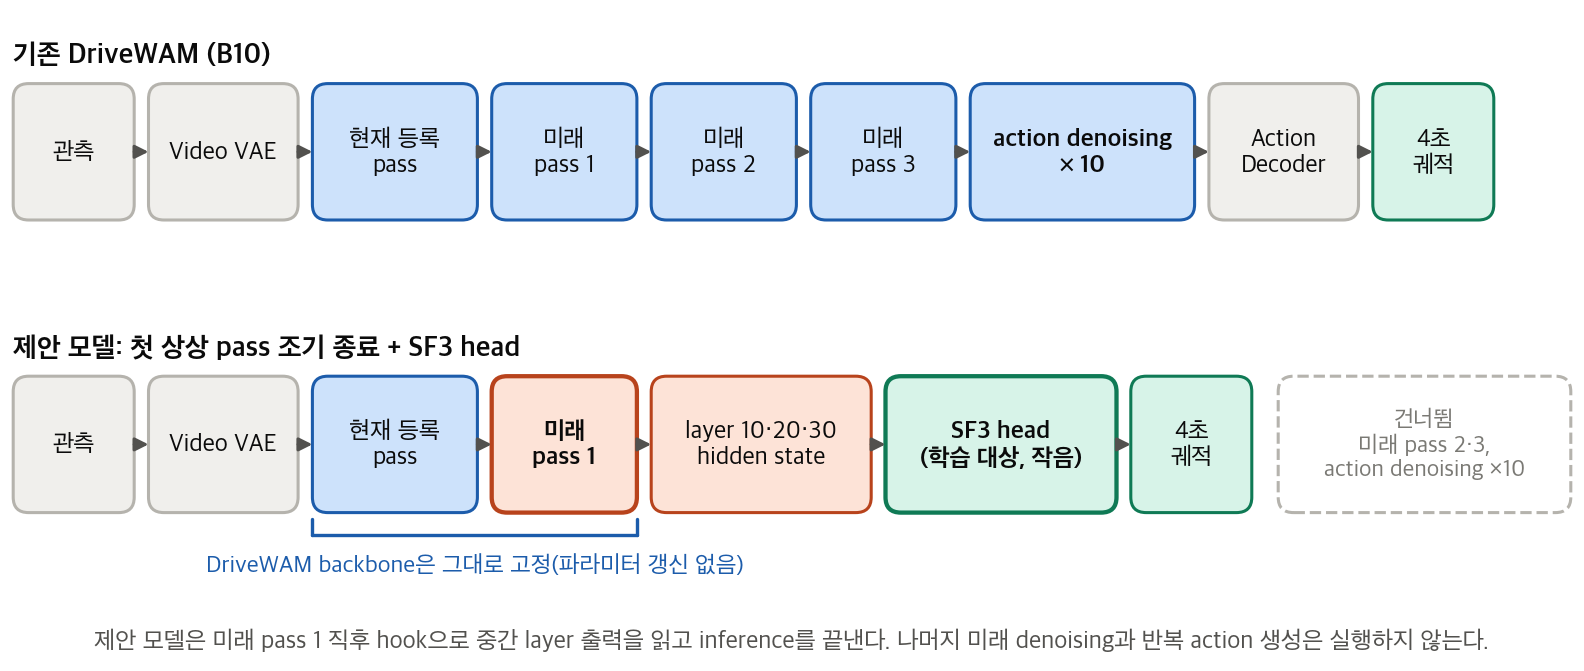
\includegraphics[width=0.68\linewidth]{fig2_compare.png}
\captionof{figure}{공식 DriveWAM 추론(위)과 제안 readout(아래). 백본은 갱신하지 않는다.}
\label{fig:overview}
\end{center}

\subsection{실험}
\textbf{설정.} NAVSIM v1.1~\cite{dauner2024navsim}: 장면 하나 $\rightarrow$ 4초 궤적 하나, 공식 PDMS. head는 navtrain 92,599장면으로 학습했고 navtest를 로그 단위로 dev 세트(3,250장면)와 잠금 final 세트(8,896장면)로 나눴다. PhysicalAI-AV~\cite{nvidia2025physicalai}: clip 하나 $\rightarrow$ teacher forcing으로 4초 chunk 5개, 공식 ADE/FDE. head는 공개 train 20k clip으로 학습, dev 세트는 val 1,000 clip, final 세트는 공식 test 1k.

\begin{center}
\small
\setlength{\tabcolsep}{5pt}
\begin{tabular}{lcc@{\hskip 14pt}ccc}
\toprule
 & \multicolumn{2}{c}{NAVSIM navtest-final} & \multicolumn{3}{c}{PhysicalAI-AV 공식 test 1k} \\
\cmidrule(lr){2-3}\cmidrule(lr){4-6}
모델 & PDMS $\uparrow$ & p50 (ms) $\downarrow$ & ADE (m) $\downarrow$ & FDE (m) $\downarrow$ & p50 (ms) $\downarrow$ \\
\midrule
DriveWAM B10 (공식)      & 89.67 & 797.9 & 0.802 & 2.384 & 837.8 \\
$B^{*}$ (dev에서 선정) & 89.65 (B02-opt) & 420.7 & 0.842 (B03-opt) & 2.362 & 434.0 \\
제안 모델 SF3-first, seed 17 & 89.25 & \textbf{189.0} & 0.750 & 2.244 & \textbf{70.9} \\
제안 모델 SF3-first, seed 29 & 89.49 & \textbf{189.0} & 0.748 & 2.244 & \textbf{70.9} \\
제안 모델 SF3-first, seed 43 & --    & --    & 0.762 & 2.287 & \textbf{70.9} \\
\bottomrule
\end{tabular}
\captionof{table}{잠금 final 세트(1회 평가). p50: RTX A5000 1장에서 결정 1회 지연의 중앙값. NAVSIM은 policy 호출 전체, PhysicalAI는 실제 기록 등록 이후의 결정 시간(dev 128 clip)을 쟀다. NAVSIM: B10 대비 $\Delta$PDMS $-0.42\,[-0.76,-0.08]$ / $-0.17\,[-0.56,+0.27]$(95\% CI).}
\label{tab:final}
\end{center}

\textbf{결과.} PhysicalAI: 모든 seed가 공식 단일 표본 B10보다 ADE($-0.040$ $\sim$ $-0.054$ m)와 FDE($-0.10$ $\sim$ $-0.14$ m)가 낮고 $B^{*}$보다 6.1배 빠르다. NAVSIM: B10보다 PDMS가 0.17--0.42점 낮고 $B^{*}$보다 2.2배 빠르다. 충돌(NC)은 0.15--0.17 개선되고 주행 가능 영역 준수(DAC)는 0.35--0.51 악화된다.
\textbf{미래 패스 하나면 충분하다}(표~\ref{tab:diag}). \texttt{first}는 두 벤치마크 모두 \texttt{current}보다 확실히 좋고, \texttt{terminal}은 \texttt{first}보다 유의한 이득이 없다. \textbf{head 학습 데이터가 많을수록 격차가 줄어든다}: NAVSIM의 B10 대비 격차는 4k에서 92.6k 장면 사이에 $-4.2$에서 $-0.4$ PDMS로 줄었다.
\begin{center}
\footnotesize
\setlength{\tabcolsep}{6pt}
\begin{tabular}{lcc}
\toprule
읽기 시점, head 학습 세트 & NAVSIM navtest-dev PDMS (seed 17 / 29) & PhysicalAI dev ADE (m, seed 3개 평균) \\
\midrule
\texttt{current}(관측만), 4k & 83.20 / 83.61 & 0.926 \\
\texttt{first}(미래 패스 1), 4k & 86.60 / 86.89 & 0.813 \\
\texttt{terminal}(미래 패스 전부), 4k & 87.34 / 86.28 & 0.825 \\
\texttt{first}, 20k & 89.36 / 90.00 & 0.762 \\
\texttt{first}, 92.6k & 90.43 / 90.58 & -- \\
DriveWAM B10 (참고) & 90.93 & 0.821 \\
\bottomrule
\end{tabular}
\captionof{table}{읽기 시점과 head 학습 데이터에 따른 dev 세트 결과. \texttt{first} 대 \texttt{current}: +3.3 PDMS, ADE $-0.11$ m(95\% CI가 0 제외).}
\label{tab:diag}
\end{center}

\textbf{한계.} 평균 오차 지표는 결정적 회귀에 유리하므로 DriveWAM보다 정확하다고 주장하지 않는다. PhysicalAI dev 세트에서 B10 표본 4개 평균과 비교하면 ADE는 대등하고 FDE는 약 0.1 m 나쁘다. 읽기 시점 비교는 4k 학습 데이터에서 했다. 코드: \url{github.com/thddydgnl/drivewam-lightweight-action-readout}.

\begin{posterrefs}
\bibitem{shi2026drivewam} C.~Shi et al., DriveWAM, arXiv:2605.28544, 2026.
\bibitem{wan2025wan} Team Wan, Wan: open and advanced large-scale video generative models, arXiv:2503.20314, 2025.
\bibitem{li2026lightwam} Z.~Li et al., Light-WAM, arXiv:2606.08242, 2026.
\bibitem{ma2026fasterwam} L.~Ma et al., Faster-WAM (deep action modules), arXiv:2608.02365, 2026.
\bibitem{zhao2026fasterwam} W.~Zhao et al., Faster-WAM (future conditioning), arXiv:2608.04404, 2026.
\bibitem{dauner2024navsim} D.~Dauner et al., NAVSIM, NeurIPS Datasets and Benchmarks, 2024.
\bibitem{nvidia2025physicalai} NVIDIA, PhysicalAI-Autonomous-Vehicles dataset, 2025.
\end{posterrefs}

\end{mdframed}

\end{document}
